%% ------------------------------------------------------------------------- %%
\chapter{Passeio de Euler}
\label{cap:passeio-euler}



Agora que vimos um algoritmo eficiente que resolve o problema do \LCA\, vamos explorar uma outra técnica que tem o mesmo tempo de complexidade. Neste capítulo estudaremos um algoritmo capaz de resolver problemas um pouco mais complexos em que, por exemplo, é necessário atualizar o valor de um nó da árvore rapidamente (diferente dos outros algoritmos em que a árvore deve ser sempre estática - isto é - sem modificações).


\section{Descrição}

Vamos imaginar que temos uma função $F(a, b)$ que devolve todos os vértices no caminho de $a$ para $b$. Para melhor ilustrar isso, considere a seguinte árvore enraizada:

\vspace{0.5cm}

\begin{figure}[htb]
\begin{center}
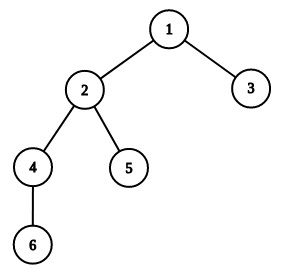
\includegraphics[width=7cm]{images/graph_euler.png}
\end{center}
\caption{\label{fig:arvore-euler}Árvore enraizada de 6 vértices}
\end{figure}

\vspace{0.5cm}

Assim, ao chamar $F(2, 3)$ a função nos retorna os vértices 2, 1 e 3.

Ao chamar $F(5, 6)$ os vértices devolvidos são 5, 2, 4 e 6.

Além disso, como de costume vamos também pré-calcular as profundidades de cada vértice de nossa árvore:

\begin{table}[htb]
\centering
\begin{tabular}{|l|c|c|c|c|c|c|}
\hline
Vértice      & 1 & 2 & 3 & 4 & 5 & 6  \\ \hline
Profundidade & 1 & 2 & 2 & 3 & 3 & 4 \\ \hline
\end{tabular}
\caption{Profundidades dos vértices da árvore acima}
\end{table}



Agora, para saber o \LCA\ entre dois nós $a$ e $b$, usaremos os vértices retornados pela chamada da função $F(a, b)$ para eles (denotaremos o conjunto destes vértices de $P(caminho)$). Afinal, pela definição o \LCA$(a, b)$ é o vértice menos profundo que contém $a$ e $b$ em sua subárvore. Isto é, o vértice menos profundo que está no caminho de $a$ até $b$.

Assim, basta verificar qual é o vértice de menor profundidade dentre os nós de $P(caminho)$: no primeiro exemplo, tal vértice é 1 - enquanto no segundo exemplo é 2. Podemos verificar que eles são, de fato, os respectivos \LCA s de seus problemas.


\section{Obtendo todos os vértices de qualquer caminho}

Previamente assumimos que existe uma função F que retorna todos os vértices do caminho entre dois nós $a$ e $b$ de uma árvore. Entretanto, ainda não estudamos como escrever esta função.

Toda vez que queremos fazer uma consulta entre dois vértices $a$ e $b$, poderíamos percorrer o caminho entre estes dois vértices visitando todos os nós entre eles um a um. Ou seja, um algoritmo linear - ineficiente para nosso problema.

Porém, podemos montar uma estrutura de dados que nos possibilita obter de maneira rápida todos os vértices no caminho entre quaisquer vértices $a$ e $b$ de uma árvore.


\subsection{Passeio de Euler}

O que faremos é "planificar"\ uma árvore, de forma que tenhamos uma sequência de vértices em uma determinada ordem.

A ideia é rodar uma DFS a partir da raiz contando um tempo crescente conforme a recursão é chamada. Considere o percurso de uma árvore usando uma DFS. Quando um nó é visitado podemos anotar o tempo que isso ocorre, de acordo com os seguintes critérios:

\begin{itemize}
    \item Anotamos o tempo em que iniciamos a busca em cada filho de um dado vértice $x$
    \item Anotamos o tempo em que terminamos a busca de todos os filhos de $x$
\end{itemize}

Entender a ideia deste algoritmo é muito mais fácil introduzindo o código e um exemplo. Vamos então apresentar a DFS que executa o algoritmo mencionado. Para cada tempo decorrido guardamos qual foi o vértice visitado naquele momento. Note que é necessário que exista uma variável global $contador$ inicializada com 1.

\vspace{10cm}

\begin{algorithm}[H]
\caption{Contando os tempos}
\begin{algorithmic}[1]
\Function{\textsc{Euler}}{vertice}
    \For{cada $filho$ em $filhos[vertice]$}
        \State $mapa[contador] \rec vertice$
        \State $contador \rec contador + 1$
        \State $Euler(filho)$
    \EndFor
    \State $mapa[contador] \rec vertice$
    \State $contador \rec contador + 1$
\EndFunction
\end{algorithmic}
\end{algorithm}


Para exemplificar usaremos novamente a árvore introduzida no início deste capítulo, já com os tempos que cada vértice guardou após a execução do código acima:

\vspace{0.5cm}

\begin{figure}[htb]
\begin{center}
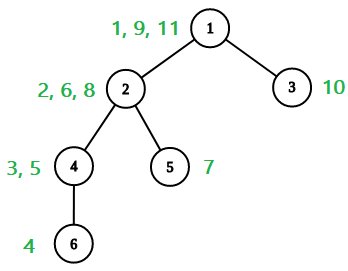
\includegraphics[width=8cm]{images/graph_euler_numbered.png}
\end{center}
\caption{\label{fig:arvore-euler2}Passeio de Euler na árvore da figura 6.1}
\end{figure}

Para fazer uma consulta basta pegar \textbf{qualquer} tempo do primeiro vértice e \textbf{qualquer} tempo do segundo vértice e retornar todos os vértices cujo tempo esteja contido neste intervalo de tempos.

Vamos simular o resultado da consulta nessa estrutura para os vértices $4$ e $5$. Vamos escolher o tempo 3 (do vértice 4) e o tempo 7 (do vértice 5). Logo, os vértices retornados são:



\begin{center}
    4, 6, 4, 2, 5    
\end{center}

Por fim, basta verificar qual desses vértices possui a menor altura - este será o \LCA. No exemplo, o vértice com tal propriedade é $2$, e de fato podemos verificar que ele é o \LCA\ entre os nós $4$ e $5$.

Note que podem ser retornados vértices que não pertencem ao caminho entre os dois nós consultados. No exemplo, o vértice $6$ não está no caminho entre $4$ e $5$ mas está contido no intervalo. Entretanto, podemos observar que a profundidade dele é maior do que a de ambos $4$ e $5$ (afinal, ele é filho de $4$) - o que nos diz que sua presença no intervalo não faz diferença para a obtenção do \LCA. Provaremos o porquê deste algoritmo sempre funcionar na seção 6.6 deste capítulo.

\section{Otimização com árvore de segmentos}

Embora agora conseguimos obter todos os vértices de qualquer caminho, ainda não conseguimos calcular de forma eficiente qual é o vértice de menor profundidade do conjunto $V$. Isto é, no pior caso temos $n$ vértices em um caminho e teríamos que percorrer todos estes nós verificando um a um qual é o de menor profundidade, levando a um algoritmo de tempo $O(n)$.

Porém, usando uma famosa estrutura de dados chamada árvore de segmentos (do inglês, \textit{segment tree}), discutida em \cite{arvore-segmentos}, conseguimos obter o vértice de menor profundidade em tempo $O(log\ n)$. Essa estrutura permite fazer consultas de operações cumulativas (adição, máximo, mínimo, etc) em um intervalo de uma lista de maneira eficiente.

Como o objetivo deste trabalho é focar exclusivamente em resolver o problema do ancestral comum mais próximo, não discutiremos em detalhes como essa estrutura funciona, tampouco escreveremos seu código. Ao invés, assumiremos que temos as seguintes funções de nossa árvore de segmentos, que armazenará as profundidas dos nós:

\begin{itemize}
    \item \textbf{Constrói(lista)}: monta uma árvore de segmentos a partir de uma lista de valores. Leva tempo $O(n)$ onde $n$ é o tamanho da lista.
    \item \textbf{Atualiza(posição, valor)}: atualiza uma posição da árvore de segmentos com o valor passado. Leva tempo $O(log\ n)$.
    \item \textbf{Consulta(esquerda, direita)}: devolve o índice da posição de menor valor no intervalo $[esquerda,\ direita]$. Leva tempo $O(log\ n)$.
\end{itemize}

Por enquanto, vamos focar na função de consulta. Ela resolve o nosso problema inicial de achar um elemento mínimo em um intervalo de maneira rápida.

Na próxima seção utilizaremos todas as funções mencionadas, juntamente com a ideia descrita na seção \textbf{Passeio de Euler} para montar a nossa estrutura completa de determinar \LCA s.

\section{Código}

Faremos uma modificação do algoritmo 8 apresentado neste capítulo. Conforme percorremos a árvore contando os tempos vamos simultaneamente construindo a árvore de segmentos. Assumiremos novamente que a variável global $contador$ foi inicializada com o valor 1.

\begin{algorithm}[H]
\caption{Passeio de Euler}
\begin{algorithmic}[1]
\Function{\textsc{Euler}}{vertice}
    \For{cada $filho$ em $filhos[vertice]$}
        \State $mapa[contador] \rec vertice$
        \State $arvoreSeg[contador] \rec profundidade[vertice]$
        \State $contador \rec contador + 1$
        \State $Euler(filho)$
    \EndFor
    \State $tempo[vertice] \rec contador$
    \State $mapa[contador] \rec vertice$
    \State $arvoreSeg[contador] \rec profundidade[vertice]$
    \State $contador \rec contador + 1$
\EndFunction
\end{algorithmic}
\end{algorithm}

Abaixo estão os resultados de $mapa$, $arvoreSeg$ e $tempo$ após a execução deste algoritmo para a árvore apresentada na descrição deste capítulo:

\begin{table}[htb]
\centering
\begin{tabular}{|l|c|c|c|c|c|c|c|c|c|c|c|}
\hline
Índice      &  1 & 2 &  3 & 4 & 5 & 6 & 7 & 8 & 9 & 10 & 11 \\ \hline
mapa        &  1 & 2 &  4 & 6 & 4 & 2 & 5 & 2 & 1 &  3 &  1 \\ \hline
arvoreSeg   &  1 & 2 &  3 & 4 & 3 & 2 & 3 & 2 & 1 &  2 &  1 \\ \hline
tempo       & 11 & 8 & 10 & 5 & 7 & 6 & - & - & - &  - &  - \\ \hline

\end{tabular}
\caption{Resultado da execução do algoritmo 9 para o exemplo}
\end{table}

Algumas observações sobre o que fizemos:

\begin{itemize}
    \item $mapa[x]$ guarda qual é o vértice visitado no instante de tempo $x$
    \item $arvoreSeg[x]$ guarda qual é a profundidade do vértice obtido ao consultar $mapa[x]$
    \item $tempo[v]$ guarda o último tempo registrado do vértice $v$ (para que depois possamos usá-lo na consulta, já que qualquer tempo nos basta) - ou seja - sempre o maior valor de $contador$
\end{itemize}

\vspace{0.5cm}

O último passo é simplesmente chamar a função \textbf{Constrói(arvoreSeg)} para montar a árvore de segmentos a partir dos valores preenchidos em $arvoreSeg$. Assim, para cada consulta temos o algoritmo abaixo:

\begin{algorithm}[H]
\caption{LCA utilizando a estrutura de Euler}
\begin{algorithmic}[1]
\Function{\textsc{LCA}}{a, b}
    \State $esquerda \rec tempo[a]$
    \State $direita \rec tempo[b]$
    \If{$esquerda > direita$}
        \State $troca(esquerda, direita)$
    \EndIf
    \State $indice \rec Consulta(esquerda,\ direita)$
    \\\hspace{5mm} \Return $mapa[indice]$
\EndFunction
\end{algorithmic}
\end{algorithm}

\section{Corretude}

Vamos mostrar que, após percorrermos a árvore de Euler anotando os tempos de cada vértice da meneira mencionada, podemos escolher \textbf{qualquer} tempo de um vértice para ser usado na hora de achar o \LCA. Em outras palavras, vamos provar que para qualquer par de tempos escolhido de $a$ e $b$, o vértice de menor profundidade do intervalo contínuo $[tempo[a],\ tempo[b]]$ da árvore de Euler será o \LCA(a, b).

\vspace{0.5cm}

Vamos assumir que o \LCA\ de dois nós $a$ e $b$ é o vértice $c$. Então, quando chamamos a DFS do Passeio de Euler partindo da raiz sabemos que vamos encontrar o vértice $c$ antes de $a$ e $b$ (afinal, ele é o \LCA\ e tem profundidade menor do que seus descendentes). Estando em $c$, vamos assumir sem perda de generalidade que a subárvore do vértice $a$ é chamada antes do que a de $b$. Assim, eventualmente $a$ ganhará um ou mais tempos. O importante é que quando a subárvore inteira de $a$ for visitada, a DFS voltará para o vértice $c$, dando a ele um novo tempo.

Logo, podemos notar que para todo tempo do vértice $a$ existe um tempo de $c$ que é maior.

Seguindo o algoritmo, quando a DFS for chamada para a subárvore de $b$, podemos notar que todos os tempos que serão eventualmente associados ao vértice $b$ serão maiores do que algum tempo de $c$.

Por fim, também é verdade que todo tempo de $b$ será estritamente maior do que todo tempo de $a$, já que a DFS só será executada para a subárvore de $b$ quando terminar integralmente de percorrer a subárvore de $a$. Então, se colocarmos os tempos de $a, b$ e $c$ numa linha temporal, temos:

\begin{center}
    $[$todos os tempos do vértice $a$, \ algum tempo do vértice $c$, \ todos os tempos do vértice $b]$
\end{center}

E por este motivo podemos escolher qualquer tempo de $a$ e qualquer tempo de $b$, pois sempre existirá um tempo do vértice $c$ contido no intervalo formado pela escolha.

\vspace{0.5cm}

Outra observação deste algoritmo é que no intervalo $[tempo[a],\ tempo[b]]$ podem existir valores associados a vértices que não necessariamente estão no caminho de $a$ até $b$. Porém, isso não é um problema devido ao fato de que todos eles serão descendentes do vértice $c$ (o \LCA\ do problema) e por isso terão profundidade estritamente maior. Como o intuito desta estrutura é nos possibilitar inferir quem é o \LCA\ verificando o vértice de menor profundidade, estes nós adicionais no intervalo não fazem diferença alguma.

\vspace{5cm}

\section{Complexidade}

A complexidade deste algoritmo é fácil de ser obtida. Vamos analisar as três partes do código:

\begin{itemize}
    \item Algoritmo 8: uma DFS com operações de tempo constante. Portanto, sua complexidade de tempo é $O(n+m)$
    \item Construção da árvore de segmentos: como discutido anteriormente, esta "função caixa-preta"\  possui complexidade de tempo $O(n)$, onde $n$ é o tamanho da árvore a ser montada
    \item Algoritmo 9: esta outra "função caixa-preta"\ possui complexidade de tempo $O(log\ n)$, onde $n$ é a quantidade de nós da árvore de segmentos. Podemos assumir que o retorno da função é executado em tempo constante já que poderíamos utilizar uma lista para armazenar o mapeamento de tempos para vértices.
\end{itemize}

Resumindo, a complexidade de tempo da construção de nossa estrutura de dados é $O(n)$, enquanto uma consulta de \LCA\ é $O(log\ n)$.